%!TEX root = ../main.tex
%%%%%%%%%%%%%%%%%%%%%%%%%%%%%%%%%%
% Links:
%
% Difficulty: Companies: 
%%%%%%%%%%%%%%%%%%%%%%%%%%%%%%%%%%

\chapter{BST Lowest Common Ancestor}
\label{ch:lowest_common_ancestor}
\section*{Introduction}
The lowest common ancestor is an important concept in graph theory and it is quite often a topic or
a fundamental building block of coding interview questions. LCA have important application in graph
theory for instance in:
\begin{itemize}
	\item computation of \textit{minimum spanning tree},
	\item finding a \textit{dominator tree}, or
	\item as a stepping stone for algorithm for \textit{network routing}, or \textit{range
	searching}.
\end{itemize}
Given a tree and two nodes $p$ and $q$, the lowest common ancestor  of $p$ and $q$, ($LCA(p,q)$) is
defined as the lowest or deepest node that has both $p$ and $q$ as descendant. In other words the
LCA is the shared ancestor or $p$ and $q$ that is the farthest from the root of the tree. 

There are
several known algorithm for finding the LCA efficiently on a generic tree, one of the most
fundamental being the one from Harel and Tarjan \cite{harel84,harel80}.
In this chapter however, we will focus on the (simpler) problem of finding the LCA for  trees of a
particular kind: binary search trees. This constraint greatly simplifies the general problem of finding LCA. 
\section{Problem statement}
\begin{exercise}
	Write a function that takes a binary search tree $T$, and two nodes $p$ and $q$ and returns
	their lowest common ancestor.

	\begin{example}
		\hfill \\
		Given the tree in Figure \ref{fig:lowest_common_ancestor:example1} the lowest common
		ancestor for nodes:
		\begin{itemize}
			\item $p = 2$, $q=12$ is node $3$
			\item $p = 12$, $q=3$ is node $12$
			\item $p = 18$, $q=1$ is the root node $13$
		\end{itemize}
		\label{ex:lower_common_ancestor:example1}
	\end{example}
\end{exercise}

\begin{figure}
	\centering
	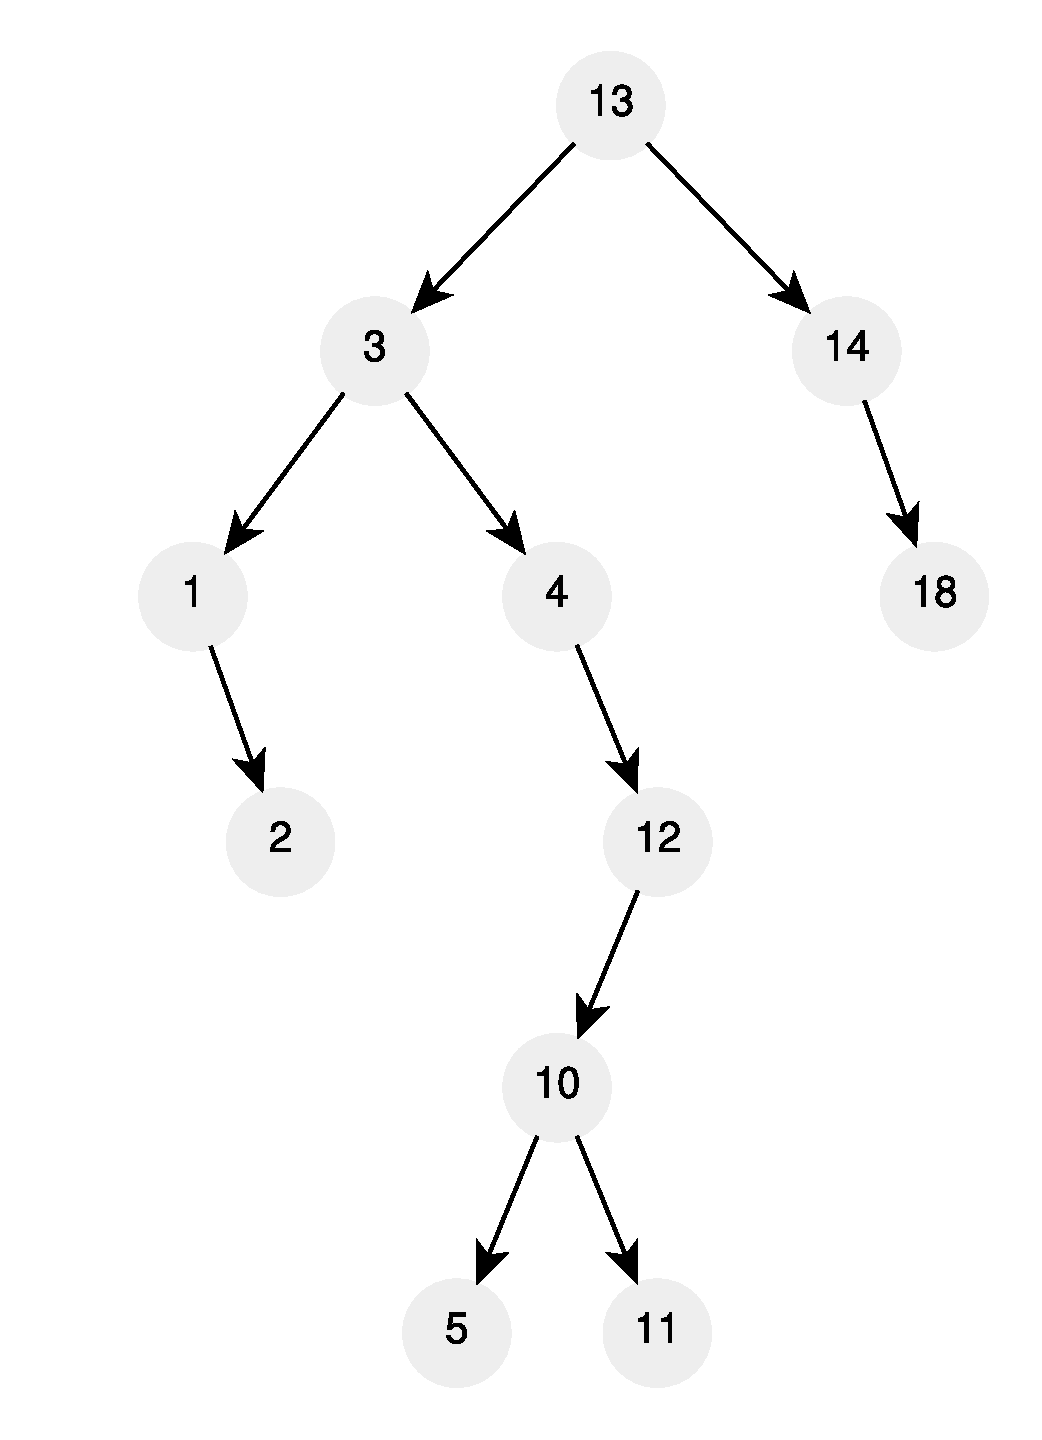
\includegraphics[width=0.5\textwidth]{sources/lowest_common_ancestor/images/example1}
	\caption[Sample short cpation]{Binary Search tree of the Example
	\ref{ex:lower_common_ancestor:example1}}.
	\label{fig:lowest_common_ancestor:example1}
\end{figure}

\section{Clarification Questions}

\begin{QandA}
	\item What to return in case the input tree is empty?
	\begin{answered}
		\textit{You can return an empty tree.}
	\end{answered}


	\item Should I check for the validity of the binary search property for $T$?
	\begin{answered}
		\textit{No, you can assume $T$ to always be a valid binary search tree.}
	\end{answered}

	\item Can I assume $p$ and $q$ to always be always present in $T$?
	\begin{answered}
		\textit{Yes}
	\end{answered}

	
\end{QandA}

\section{Discussion}
\label{lowest_common_ancestor:sec:discussion}
Based on the definition of LCA one of the simplest solution possible would be to compute the path
from the root to $p$ and $q$ as store them as two separate lists of nodes: $P_q$ and $P_p$. We can
then compare these lists and notice that they will match up until a certain point, say up to the
$k^{th}$ node of the path. After that the lists do not match anymore.
Therefore the $k^{th}$ element of the list is the LCA for $p$ and $q$. 
For instance w.r.t the tree in Figure \ref{fig:lowest_common_ancestor:example1}
the paths from the root to the nodes $5$ and $2$ are the following, respectivey:
	\begin{flalign}
		&P_5 = \{\mathbf{13,3},4,12,10,5\} \\
		&P_2 = \{\mathbf{13,3},1,2\} 
	\end{flalign}
As you can see they match up to node $3$ that is indeed their LCA.

If we try the same approach for the nodes $5$ and $11$ we have that their respective paths from the
root are:
	\begin{flalign}
		&P_5 = \{\mathbf{13,3,4,12,10},5\} \\
		&P_1 = \{\mathbf{13,3,4,12,10},11\} 
	\end{flalign}
$P_5$ and $P_{11}$ match up to until the penultimate node ($10$). Therefore, their LCA is  node $10$.

This approach is correct and it is easily implementable, and its time and space complexity
is $O(k)$ where $k$ is the height of $T$ (which for unbalanced trees might be proportional to the
number of nodes in $T$). Listing \ref{list:lowest_common_ancestor_paths} show an implementation of
the idea above. 

\begin{minipage}{\linewidth}
	\lstinputlisting[language=c++, caption={LCA solution based on the difference of paths from the root.},label=list:lowest_common_ancestor_paths]{sources/lowest_common_ancestor/lowest_common_ancestor_solution2.cpp}
\end{minipage}

This approach is however not optimal as we waste unnecessary space for storing entire paths.
This is not really necessary as we only really care about the last node that is common. 
One way to avoid memorizing the entire paths is to find the path for both $p$ and $q$ simultaneously
and only remember the last node we visited. It as some point of this visit we find that the the next
node to visit for $p$ is  different from the direction of the search for $q$ wants us to go, we can
stop as this is the point where the paths for $p$ and $q$ diverge. We can therefore return the last
element that was common. Despite the fact this approach does not improve the time complexity w.r.t
to the other solution, we have in this case only a constant space usage which is a very good
improvement compared to the linear space complexity for Listing
\ref{list:lowest_common_ancestor_paths}. This optimized version is shown in Listing
\ref{list:lowest_common_ancestor_paths_optimized}.

\begin{minipage}{\linewidth}
	\lstinputlisting[language=c++, caption={Space optimized version of Listing \ref{list:lowest_common_ancestor_paths} },label=list:lowest_common_ancestor_paths_optimized]{sources/lowest_common_ancestor/lowest_common_ancestor_solution3.cpp}
\end{minipage}


We can however simplify the implementation shown in Listing
\ref{list:lowest_common_ancestor_paths_optimized} by rewriting it such that it runs iteratively
rather than recursively. Listing \ref{list:lowest_common_ancestor_iterative} shows this iterative version which starts at the root of $T$
and keep navigating the tree until by moving left or right until the direction of the search for
both $p$ and $q$ is the same. When the path diverges we can stop and return the current node which
is the lowest node shared node in the paths from the root to $p$ and $q$

\begin{minipage}{\linewidth}
	\lstinputlisting[language=c++, caption={Iterative solution to the problem of finding the LCA in a binary search tree.},label=list:lowest_common_ancestor_iterative]{sources/lowest_common_ancestor/lowest_common_ancestor_solution1.cpp}
\end{minipage}
